\documentclass[12pt, twoside]{article}
\usepackage[francais]{babel}
\usepackage[T1]{fontenc}
\usepackage[latin1]{inputenc}
\usepackage[left=1cm, right=1cm, top=8mm, bottom=8mm]{geometry}
\usepackage{float}
\usepackage{graphicx}
\usepackage{array}
\usepackage{multirow}
\usepackage{amsmath,amssymb,mathrsfs}
\pagestyle{empty}
\begin{document}

\begin{flushright}
$2^{de}5$
\end{flushright}

\section*{\center{Mini Devoir Maison 1 (seconde chance)}}

\textit{Devoir pour les retardataires � rendre ce samedi 11 octobre dernier
d�lai.}



\bigskip
\textbf{Exercice:}


 Soit $(d)$ la droite gradu�e de rep�re $(OI)$. $OABI$ est un
carr� de c�t� $1$. $OACD$ est un rectangle tel que $OD=2$. 


$\mathcal{C}_{1}$
est le cercle de centre $O$ et de rayon $OB$. $\mathcal{C}_{2}$
est le cercle de centre $O$ et de rayon $OC$. On note $E$ et $F$ les points
d'intersections de $\mathcal{C}_{1}$ et de $(OI)$. $E$ a pour abscisse $x$. On
note $G$ et $H$ les points d'intersections de $\mathcal{C}_{2}$ et de $(OI)$.
$G$ a pour abscisse $y$.
\begin{enumerate}
  \item \begin{enumerate}
          \item Que vaut $OB$?
          \item En d�duire la valeur de $x$.
          \item Quelle est la nature de $x$?
\end{enumerate}
\item \begin{enumerate}
        \item Calculer $OC$.
        \item En d�duire la valeur de $y$.
        \item Quelle est la nature de $y$?
\end {enumerate}
\item En d�duire la valeur de l'abscisse de $F$ et celle de $H$. Justifier.
\end{enumerate}


\begin{center}
	  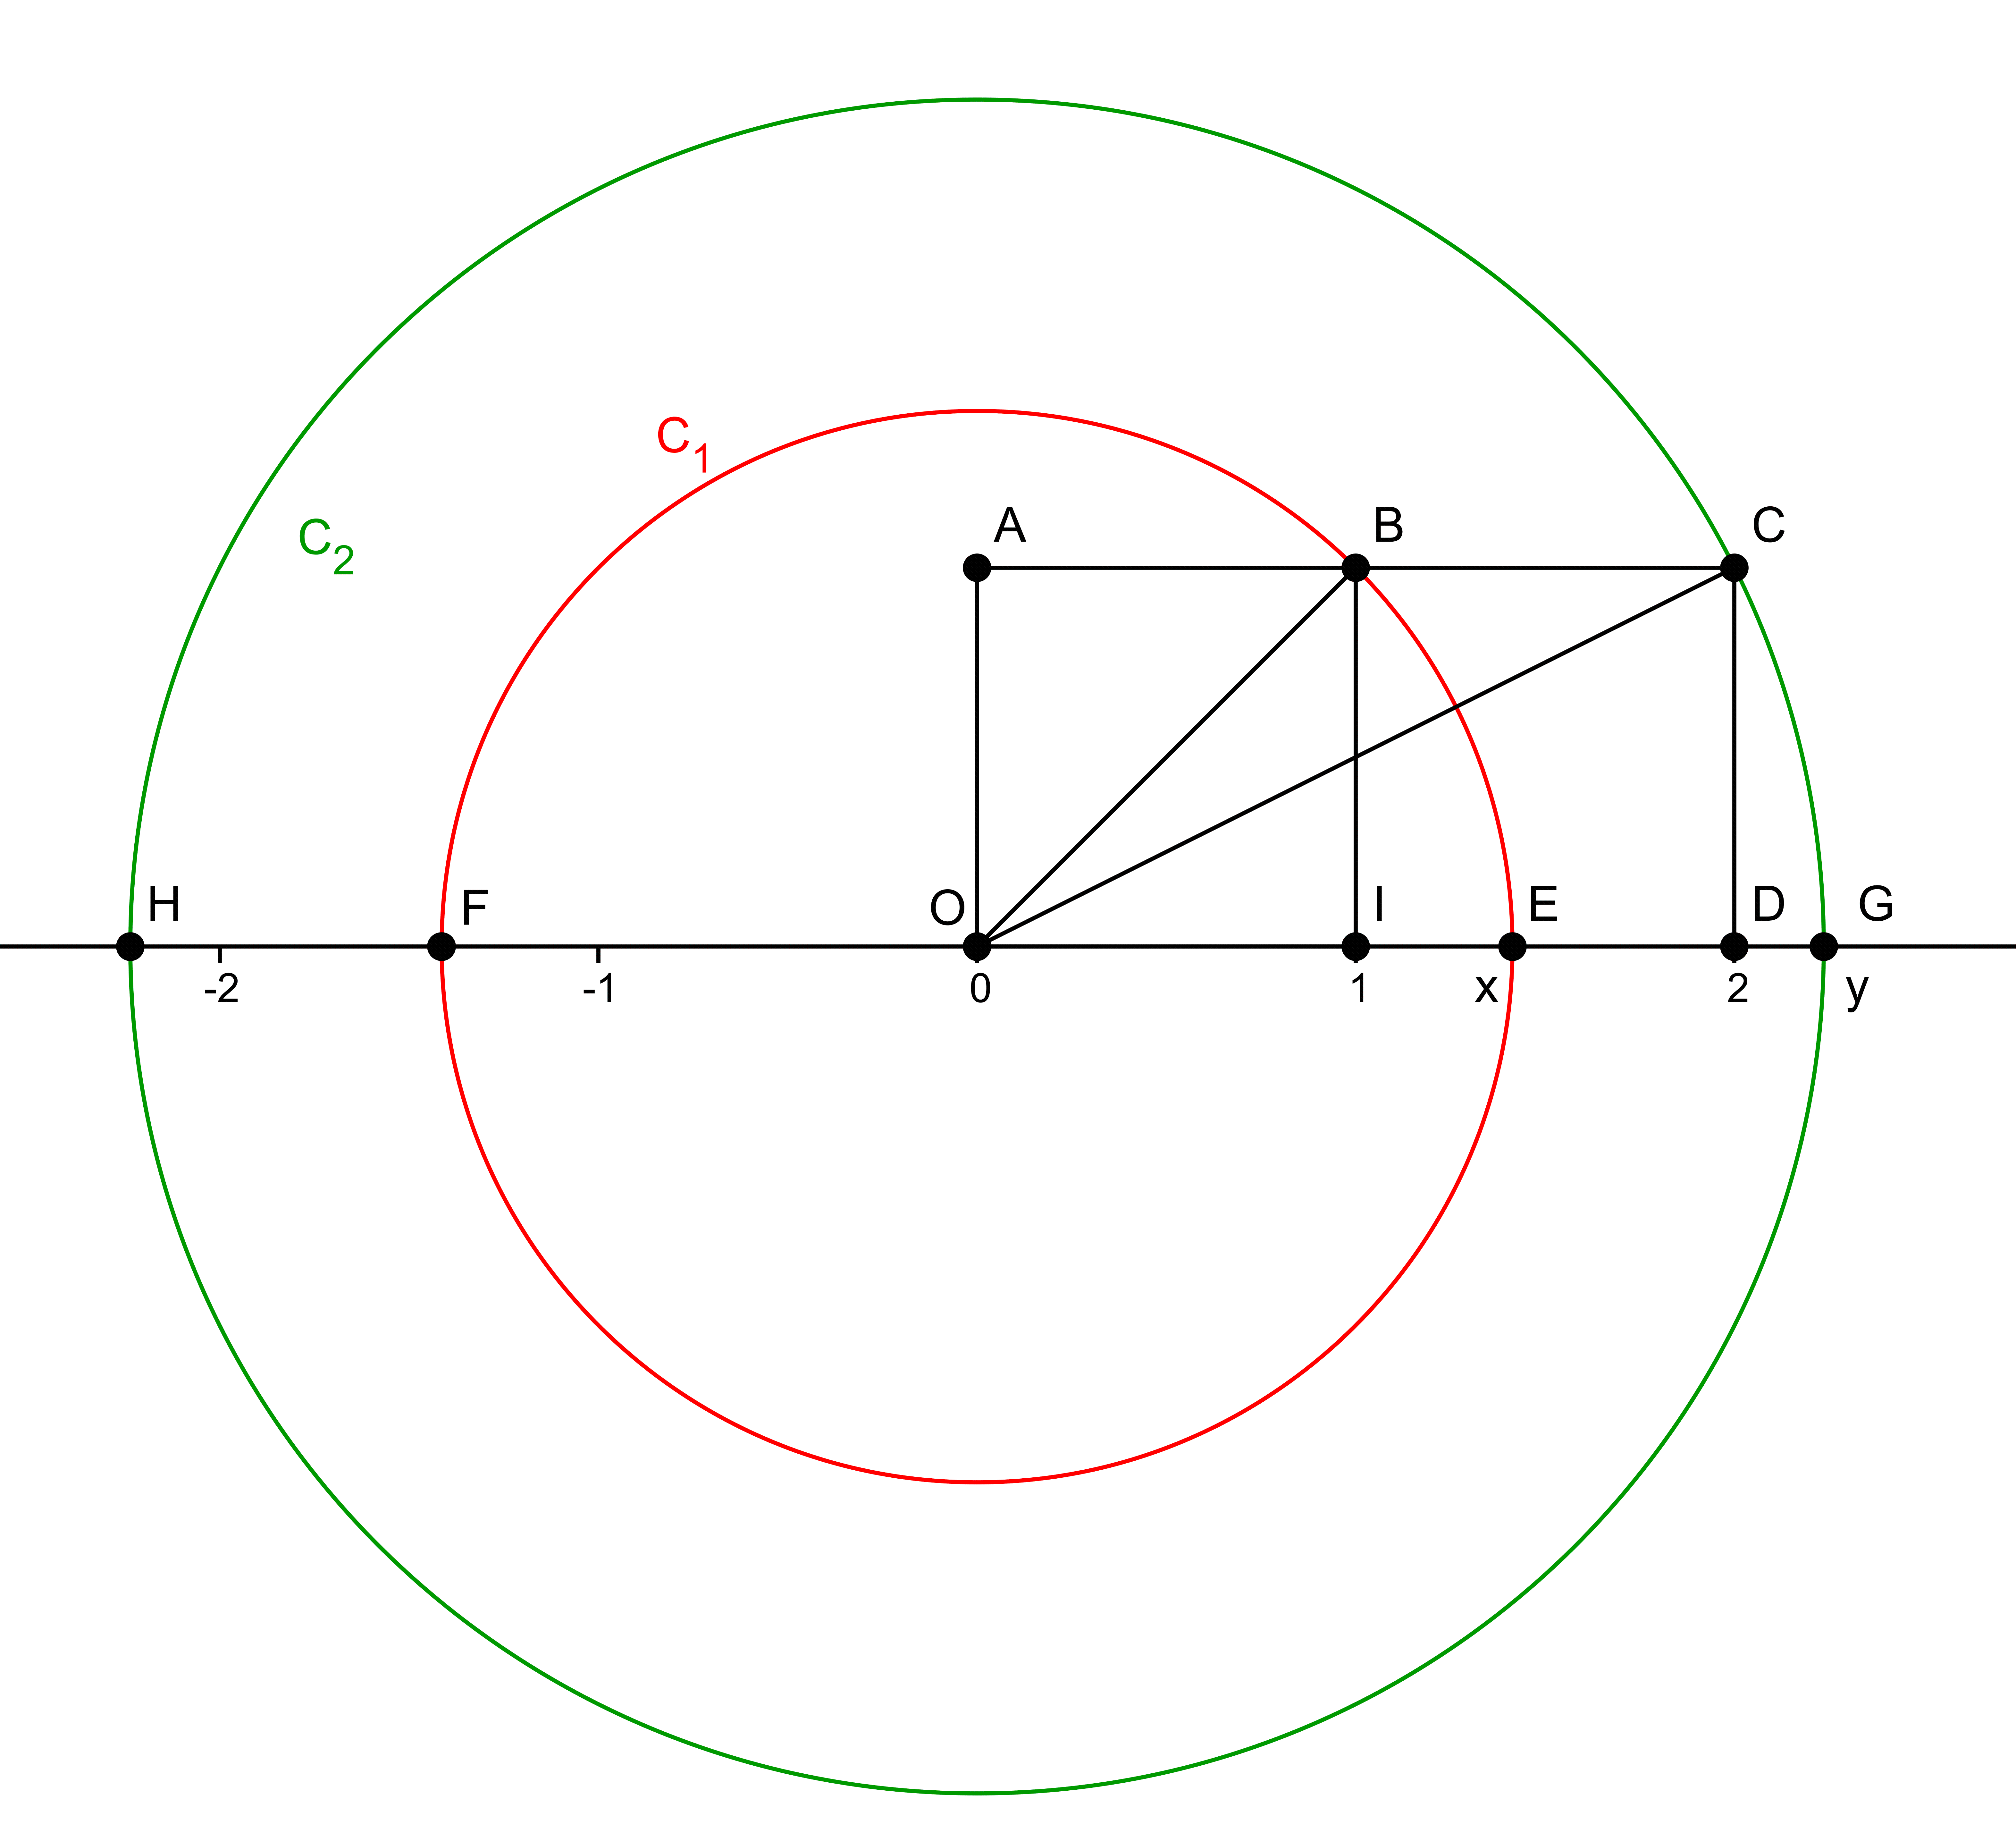
\includegraphics[width=9cm]{image/miniDM1bis.png} 
\end{center}
\end{document}
